\section{Relationale Datenbanksprachen}
\label{sec:sql}

\textbf{SQL-Kern}
\begin{items}
	\item \underline{select} \\*
		Projektionsliste \\*
		Attribute, arithmetische Ausdrücke, Aggregatfunktionen \\*
		\textbf{select distinct}: keine Dopplungen\\*
		Umbenennungen: \lstinline[language=sql]{select Preis * 1.44 as DollarPreis }
	\item \underline{from} \\*
		Zu verwendende Relationen, Umbenennungen\\*
		Orthogonalität: Wiederum SFW-Block möglich\\*
		\lstinline[language=sql]{select * from (select [...]) where [...] }
	\item \underline{where} \\*
		Selektions- und Verbundbedingungen, \\*
		geschachtelte Anfragen (wieder SFW-Block)
	\item \underline{group by} \\*
		Gruppierung für Aggregatfunktionen
	\item \underline{having} \\*
		Selektionsbedingungen an Gruppen
\end{items}

\textbf{from - Mehrere Relationen}
\begin{items}
	\item Bei mehr als einer Relation: \textbf{Kartesisches Produkt}
	\item Kommagetrennt oder als expliziter Operator:
	\begin{lstlisting}[language=sql]
select * from Kuenstler K, Titel T
select * from Kuenstler cross join Titel
	\end{lstlisting}
\end{items}

\textbf{Natürlicher Verbund}
\begin{items}
	\item Automatischer Equi-Join auf allen übereinstimmenden Spalten, diese erscheinen nur ein mal in der Ergebnisrelation
	\begin{lstlisting}[language=sql]
select * from Kuenstler natural join Titel
	\end{lstlisting}
\end{items}

\textbf{Theta-Join}
\begin{items}
	\item Verbund über Verbundsbedingungen
	\begin{lstlisting}[language=sql]
select * from Kuenstler 
	join Titel on Kuenstler.KID = Titel.KID
	\end{lstlisting}
	\item Beispiel: \(  \text{Auto} \bowtie_{AutoPreis > BootPreis} \text{Boot} \)
\end{items}

\textbf{Outer, Left, Right Join}
\begin{items}
	\item Dangling Tuples übernehmen und mit Nullwerten füllen
	\begin{figure}[H]\centering\label{SQLJoin}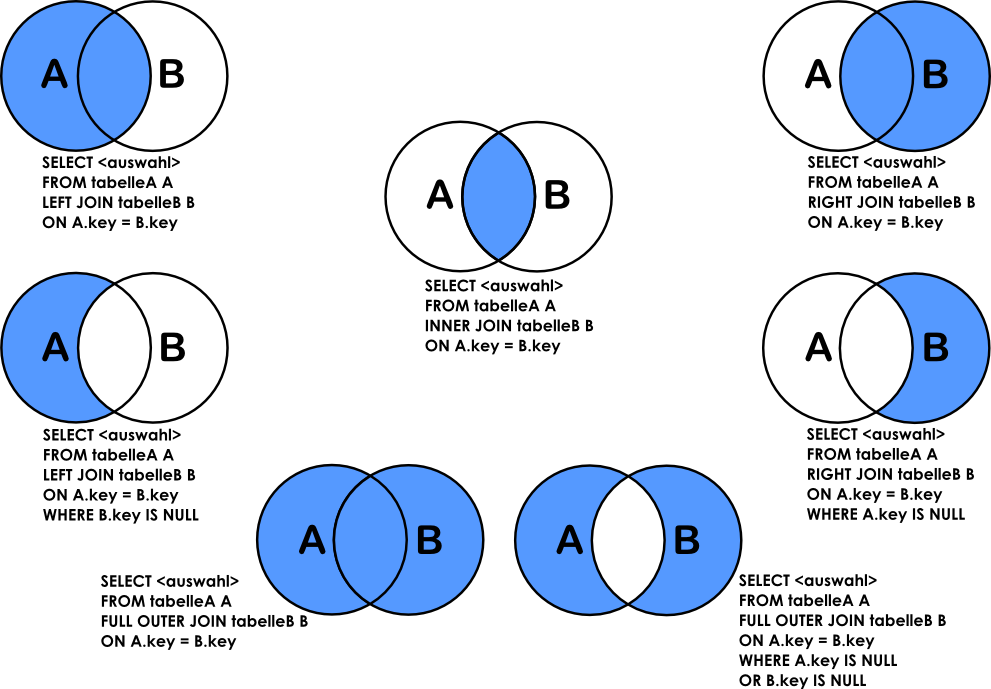
\includegraphics[width=0.4\textwidth]{SQLJoin}\end{figure}
\end{items}

\textbf{Self-Join}
\begin{items}
	\item Kartesisches Produkt einer Tabelle mit selbst
	\begin{lstlisting}[language=sql] 
	select * from SNUser eins, SNUser zwei
	where eins.Alter < zwei.Alter
	\end{lstlisting}
	Vierspaltiges Ergebnis:
	\begin{lstlisting}[language=sql]
eins.Name, eins.Vorname, zwei.Name, zwei.Vorname
	\end{lstlisting}
	\item Anwendungen: Vergleichen oder Zählen von Wertemengen
\end{items}

\newpage

\textbf{where}
\begin{items}
	\item Konstanten-Selektion: \\*
	\lstinline[language=sql]{select * from Buecher where Buecher.Titel = "Titel"}
	\item Verbundbedingung bei Cross-Join (Attribut-Selektion):
	\begin{lstlisting}[language=sql]
select Buecher.Titel, Buecher_Stichwort.Stichwort
	from Buecher, Buecher_Stichwort
	where Buecher.ISBN = Buecher_Stichwort.ISBN
	\end{lstlisting}
	\item \lstinline[language=sql]{like}: Ungewissheitsselektion
	(\lstinline[language=sql]{where name like "C\%"})\\*
	'\%' -- Beliebig viele Zeichen $\qquad$ '\_' -- Genau ein Zeichen
	\item \lstinline[language=sql]{and, or, not, is null}
	\item \lstinline[language=sql]{in}: \lstinline[language=sql]{where ISBN in (select ISBN from Empfiehlt)}
\end{items}

\textbf{Verzahnt geschachtelte Anfragen}
\begin{items}
	\item In der inneren Anfrage Attribute aus der äußeren verwenden
	\begin{lstlisting}[language=sql]
select Nachname from Personen
where 1.0 in (select Note from Prueft
	where PANr = Personen.PANr)
	\end{lstlisting}
	\item \lstinline[language=sql]{Exists}: Test, ob Ergebnis der inneren Anfrage nicht leer ist
	\begin{lstlisting}[language=sql]
select ISBN from Buch
where exists (select * from Ausleihe
	where Invnr = Buch.Invnr)
	\end{lstlisting}
\end{items}

\textbf{Mengenoperationen}
\begin{items}
	\item Übernimmt Attributnamen des linken Operanden
	\item Vereinigung
	\begin{lstlisting}[language=sql]
select A, B, C from R1 union [all]
	select A, C, D from R2
	\end{lstlisting}
	\item \lstinline[language=sql]{union all}: Duplikate werden behalten
	\item Differenz: \lstinline[language=sql]{except}
	\item Durchschnitt: \lstinline[language=sql]{intersect}
\end{items}

\textbf{Aggregatfunktionen}
\begin{items}
	\item Prinzip: Berechnung eines Werts aus Werten eines Attributs\\*
		\lstinline[language=sql]{ sum([all / distinct] Attributname) }
	\item Standard SQL: \lstinline[language=sql]{count(), sum(), min(), max(), avg()}
	\item Speziell: \lstinline[language=sql]{count(*)}
	\item Modifikatoren: \lstinline[language=sql]{all / distinct} (Voreinstellung: all)
\end{items}

\textbf{Group by}
\begin{items}
	\item Gruppierung G: Für gleiche G-Werte werden Resttupel in Relation gesammelt, darauf dann Aggregatfunktionen angewendet
	\item
	\begin{lstlisting}[language=sql]
select Marke, sum(Anzahl)
	from Zulassungen
	group by Marke
	\end{lstlisting}
	\item \textbf{Wichtig:} Jedes Select-Attribut muss entweder Gruppiert oder Aggregiert werden!
	\item \lstinline[language=sql]{having}: Bedingung auf gruppierter Relation
	\begin{lstlisting}[language=sql]
select PANr, sum(Entlohnung)
	from anstellungen
	group by PANr
	having sum(entlohnung) > 10000
	\end{lstlisting}
	
	\item
	\begin{lstlisting}[language=sql]
select Matrikelnr from Pruefung
	group by Matrikelnr
	having avg(Note) < (select avg(Note) from Pruefung)
	\end{lstlisting}
\end{items}

\newpage

\textbf{Quantoren}
\begin{items}
	\item \lstinline[language=sql]{any/some} (äquivalent):
	\begin{lstlisting}[language=sql]
select PANr, ImmaDatum
	from Studenten
	where MatNr = any (select MatNr from Prueft)
	\end{lstlisting}
	\item \lstinline[language=sql]{all}:
	\begin{lstlisting}[language=sql]
select Name from Kunde, Bestellung
	where Kunde.id = Bestellung.KundeID
	and bestellwert > ALL (SELECT avg(bestellwert) 
		from Bestellung group by KundeID)
	\end{lstlisting}
	\item Aber: Anwendbarkeit eingeschränkt, z.B. kein Vergleich auf Mengengleichheit
\end{items}

\textbf{order by}
\begin{items}
	\item Menge von Tupeln $\leadsto$ Sortierte Liste
	\begin{lstlisting}[language=sql]
select MatNr, Note from Prueft
	where V_Bez = 'DBS'
	order by Note [asc / desc], MatNr
	\end{lstlisting}
	\item Aufsteigend (\lstinline[language=sql]{asc}, Standard) oder Absteigend (\lstinline[language=sql]{desc})
	\item \textbf{Wichtig}: Sortier-Attribut(e) müssen in Select vorkommen!\\*
	Denn: Sortierung wird auf das Ergebnis der vorherigen SFW-Anfrage angewendet.
\end{items}

\textbf{Nullwerte}
\begin{items}
	\item Vergleiche mit Nullwert: \lstinline[language=sql]{unknown} statt \lstinline[language=sql]{true} oder \lstinline[language=sql]{false} \\*
	\( \leadsto A=A \) keine Tautologie!
	\item Deshalb \textbf{nicht gleich}: \lstinline[language=sql]{select * from Person} und \\* \lstinline[language=sql]{select * from Person where Name = Name}\\*
	(Letzteres eliminiert Tupel mit Name = null)
\end{items}

\textbf{Änderungsoperationen}
\begin{items}
	\item \textbf{Insert}
	\begin{lstlisting}[language=sql]
insert into relation [(attribut1, ...)]
	values (wert1, ...)
	\end{lstlisting}
	
	\item Auch SQL-Anfragen als Wert möglich.
	\begin{lstlisting}[language=sql]
insert into Kunde (select LName, LAdr, 0 from Lieferant)
	\end{lstlisting}
	
	\item \textbf{Update}
	\begin{lstlisting}[language=sql]
update relation set attribut1 = wert, ... 
	[where bedingung]
	\end{lstlisting}
	
	\item \textbf{Delete}
	\begin{lstlisting}[language=sql]
delete from relation [where bedingung]
	\end{lstlisting}
\end{items}

\begin{fragen}
	\begin{enumeration}
		\item Formulieren diverser (komplexer) SQL-Anfragen
		\item Vorgegebene geschachtelte Anfrage als nicht-geschachtelte schreiben
		\item Welche Join-Varianten kennen Sie?
		\item Geben Sie ein Beispiel an, in dem ein Self-Join sinnvoll ist.
		\item Was ist der Zusammenhang zwischen Vereinigung und Outer Join?
		\item Was ist eine Umbenennung im SQL-Kontext? Wann wird sie gebraucht?
		\item Geben Sie ein sinnvolles Beispiel für eine Anfrage an, die eine having-Klausel hat.
		\item Geben Sie ein Bespiel für eine Anfrage mit einer having-Klausel an, bei der man
		\begin{enumeration}
			\item die Klausel durch eine where-Klausel ersetzen kann,
			\item das nicht kann.
		\end{enumeration}
		\item Erläutern Sie, warum im SQL-Kontext ``A==A'' keine Tautologie ist.
	\end{enumeration}
\end{fragen}